%======================================================================
\chapter{Background and Related Work}
%======================================================================

%\section{Natural Language Processing?}

%\subsection{Word Representations}
%
%Word representations are an integral building block of natural language processing applications.
%%The underlying problem concerns how to convert arbitrary alphanumeric representations into a format that can be represented on and processed by computers.
%The simplest approach to represent words may be to first pre-process them, e.g: with lemmatization, and then to map them to unique word IDs, thereby retrieving words with a dictionary lookup.
%However, this approach introduces a misleading notion of ordering among the words as indicated by their IDs, which does not work well with deep neural models.
%This shortcoming can be overcome with a one-hot encoding scheme where a word is represented as a vocabulary-sized vector with only the index corresponding to the word ID is set to 1 and the rest to 0.
%On the other hand, this approach comes at the cost of a large space requirement given the potentially massive sparse vectors required to represent words.
%More importantly, neither approach captures an intrinsic notion of similarity between different words; all words are orthogonal to each other in the one-hot encoding representation space.
%Intuitively, words are treated as discrete independent entities, as in exact matching methods in information retrieval, without considering their interaction with other words in the vocabulary, especially in their context.
%
%Given that the particular choice of word representations has a significance influence on the overall performance of an NLP task, learning word representations has been an active research effort in NLP for decades, spanning both non-neural \cite{ando2005framework, blitzer2006domain} and neural \cite{mikolov2013distributed, pennington2014glove} methods.
%This paradigm represents words as low-dimensional continuous feature vectors, called word embeddings, that embody hidden semantic or syntactic dependencies.
%Word embeddings can be learned from scratch for a specific corpus or pretrained over large corpora and reused, leading to significant improvements over the former \cite{turian2010word}.
%Some of the most popular pretrained English word embeddings include word2vec \cite{mikolov2013distributed} trained on  Google News, GloVe \cite{pennington2014glove} on Common Crawl, Wikipedia and Twitter, and fastText \cite{bojanowski2017enriching} on English webcrawl and Wikipedia.
%In order to leverage the context of each word, word2vec represents each word as 300-dimensional vectors based on neighbouring words in a given window with a skip-gram model.
%GloVe instead exploits the co-occurrence of words across the entire corpus rather than individual context windows to build 25 to 300-dimensional word embeddings.
%fastText takes a slightly different approach with skip-gram models than word2vec by representing each word as a bag-of-characters n-grams.
%These word embeddings enable semantic matching across multiple levels in neural networks, including the neural document retrieval methods introduced in Section \ref{neural-retrieval}

\section{Pretrained Language Models}
\label{lm}

Natural language processing tasks have traditionally been addressed with supervised learning on task-specific datasets.
Due to the relatively small size of such datasets, training deep neural networks in this manner introduces the risk of overfitting on the training data and lack of generalization across different datasets.
With the increasing availability of large corpora, pretrained deep language models have been rapidly gaining traction among NLP researchers.
%, rendering the previous common practice mostly \myworries{obsolete?}.
Language model pretraining has proven extremely effective on many natural language processing tasks ranging from machine translation to reading comprehension.
\myworries{Conditional probabilities for LM, equation?}
The underlying assumption in applying pretrained language models to downstream NLP tasks is that language modeling inherently captures many facets of language such as resolving long-term dependencies \cite{DBLP:journals/corr/LinzenDG16}, hierarchical patterns \cite{DBLP:journals/corr/abs-1803-11138}.
%In general, these models work by LSTM-based or transformer-based language models on large corpora
In general, pretrained language models can be applied to downstream tasks in one of two ways: ``feature-based'' and ``fine-tuning''.

\subsection{Feature-based Approaches}

The feature-based approach, such as ELMo \cite{peters2018deep}, employs deep pretrained representations learned with language modeling as additional features in task-specific architectures.
This approach has the advantage of being easily incorporated into existing models with significant improvements in performance.
%\myworries{Advantages?}
ELMo \cite{peters2018deep} extends traditional word embeddings to learn context-sensitive features with a deep language model.
Therefore, instead of taking the final layer of a deep BiLSTM (Bidirectional Long Short-Term Memory) as a word embedding, ELMo embeddings are learned as a function of ``all'' the internal states of a deep BiLSTM language model.
\myworries{Describe BiLSTM?}
This approach is motivated by a thread of work in NLP that suggests that the higher levels capture context \cite{melamud2016context2vec} and meaning while the lower levels learns syntactic features well \cite{belinkov2017neural}.
While traditional pretrained word embeddings like GloVe \cite{pennington2014glove} cannot differentiate between homonyms, ELMo generates different embeddings for them based on their context.
The embeddings are constructed as a shallow concatenation of independently trained left-to-right and right-to-left models.
Peters at al. \cite{peters2018deep} show that integrating these deep contextualized embeddings learned with ELMo into task-specific architectures significantly improves over the original performance in six NLP tasks, including question answering on SQuAD \cite{rajpurkar2016squad} and sentiment analysis on the Stanford Sentiment Treebank (SST-5) \cite{socher2013recursive}.

\subsection{Fine-tuning Approaches}

The more popular fine-tuning approach is inspired by the recent trend in transfer learning.
These models are first pretrained with respect to a language modeling objective, and then applied to downstream NLP tasks by ``freezing'' their last layer, and ``fine-tuning'' on external data for the specific task with minimal task-specific parameters.
Despite its simplicity, this approach has been shown to greatly boosts the performance of many NLP tasks \myworries{Examples?}.
%Not only does this approach introduce only a few task-specific parameters to optimize, but it also greatly boosts the performance of many NLP tasks given the rich semantic expressiveness introduced by the pretrained language model.

Radford et al. \cite{radford2019language} claim that this phenomenon occurs because language models inherently capture many NLP tasks without explicit supervision.
\myworries{GPT to GPT2}
Therefore, they propose Generative Pretrained Transformers (GPT-2) to perform zero-shot task transfer on multiple sentence-level tasks from the GLUE benchmark \cite{wang2018glue} with impressive results.
\myworries{Difference from ELMo?}
\myworries{Explain transformers? Separate section at the beginning?}
At the core of GPT-2 lies a multi-layer left-to-right transformer \cite{vaswani2017attention} decoder, with each layer consisting of a multi-head self-attention mechanism and fully connected feed-forward network \cite{radford2018improving}.
The large capacity of the transformer is exploited by pretraining it on Google BookCorpus dataset \cite{zhu2015aligning} where long contiguous spans of text allow the transformer to condition on long-range information.

\begin{figure}[b!]
\centering
  \includegraphics[width=5in]{bert-arch.png}
\caption{BERT Models.}
\label{fig:bert}
\end{figure}

Bidirectional Encoder Representations from Transformers (BERT)~\cite{devlin2018bert} has introduced a novel way to pretrain bidirectional language models, and has since enjoyed widespread popularity across the NLP community.
Standard language models, such as in OpenAI's GPT-2~\cite{radford2019language}, could not be conditioned on bidirectional context as this would cause the model to apply self-attention on the current token in a multi-layered context.
BERT enables bidirectional language modeling by conditioning on both left and right context in all layers by employing a new pretraining objective called ``masked language model'' (MLM).
Conceptually, MLM randomly masks some of the input tokens, i.e: 15\% of tokens in each sequence, at random with the goal of predicting the masked tokens based only on their left and right context.
The final hidden vectors corresponding to the masked tokens are then fed into a softmax layer over the vocabulary as in a standard language model.
This objective allows the representation to fuse both left and right context, which is crucial for token-level tasks such as question answering according to the authors.
Ablation studies confirm that the bidirectional nature of BERT is the single most important factor in its performance.
\myworries{Comparison image?}

In additional to the novel language modeling approach, Devlin et al. \cite{devlin2018bert} also propose a ``next sentence prediction'' task for applications that require an understanding of the relationship between two sentences, such as question answering or language language inference.
Essentially, this trains a binary classifier to determine whether or not one sentence follows another sentence.
\myworries{Details? May even add example in the paper?}
Figure \ref{fig:bert} visualizes the input and output for fine-tuning BERT for a ``sentence pair classification'' model.

The underlying model architecture of BERT is a multi-layer bidirectional transformer \cite{vaswani2017attention}.
\myworries{What about small?}
The larger BERT model has 24 layers each with 1024 hidden nodes, and 16 self-attention heads in total.
%As expected, optimizing this objective requires a very complex model:\ for example, the larger BERT model requires around 340 million parameters be optimized.
%In fact, training this model end-to-end takes four days to complete even on 16 high-end tensor processing units (TPUs)~\cite{devlin2018bert}.
%Fortunately, it is possible to benefit from these models by simply fine-tuning on task-specific data.
BERT is pretrained on the union of Google BookCorpus \cite{zhu2015aligning} (800M words) and English Wikipedia (2,500M words).
\myworries{More details?}

The input representation for BERT is formed by concatenating the token with segment and position embeddings.
The words are represented with WordPiece embeddings \cite{wu2016google} with a vocabulary of 30,000 tokens.
Originally proposed for segmentation problem in Japanese and Korean, the WordPiece model is used to divide words into small sub-word units in order to handle rare or out-of-vocabulary words more effectively.
The input to BERT may contain a single sentence or a sentence pair separated by the meta-token \texttt{[SEP]}, i.e: separator.
Each sequence is prepended with \texttt{[CLS]}, corresponding to the ``class'' meta-token, whose final hidden state can be used for classification tasks.
Positional embeddings are learned -- not hard-coded -- for up to 512, which is the maximum input size allowed by BERT.

To fine-tune BERT for classification tasks, a single-layer neural network is added to the end of this network with the class label as the input, and label probabilities are computed with softmax.
The parameters of this layer and BERT are fine-tuned jointly to maximize the log-probability of the correct label.
For span-level and token-level prediction tasks, the final step needs to be modified to account for multiple tokens.

BERT has been applied to a broad range of NLP tasks from sentence classification to sequence labeling with impressive results.
\myworries{Examples?}
Most relevant to the task of document retrieval, applications of BERT include BERTserini by Yang et al. \cite{yang2019end} which integrated BERT with Anserini for question answering over Wikipedia by fine-tuning BERT on SQuAD, and Nogueira et al. \cite{nogueira2019passage} who adopted BERT for passage reranking over MS MARCO.

\section{Document Retrieval}

\subsection{Non-neural Document Retrieval}
\label{non-neural-retrieval}

Traditional document retrieval techniques have evolved from the simple Boolean model to probabilistic models such as the Binary Independence Model over time to increase the matching effectiveness.
While these methods perform reasonably well for consistently short text like titles or abstracts, they have fallen short with the development of modern text collections with highly variable lengths \myworries{like the TREC collections}.
To this end, Okapi BM25 (commonly dubbed BM25) was developed as a bag-of-words ranking function that is sensitive to term frequency and document length without introducing too many additional parameters \cite{jones2000probabilistic}.
BM25 implementations define two parameters for term frequency saturation and field-length normalization, respectively.
Intuitively, BM25 pays more attention to the rarer terms in a query by increasing their term weight while dampening the matching signal for words that occur too frequently in a document with a term saturation mechanism.
Term weights are also normalized with respect to the document length \myworries{to ...}.

In addition to a term weighting scheme, query expansion has also been found to improve retrieval effectiveness by increasing recall.
Unlike manual relevance feedback, pseudo relevance feedback allows for automatic local analysis without extended interaction with the user.
RM3 is one such pseudo-relevance feedback mechanism where the original query is expanded by adding the top terms that appear in the contents of top $ k $ most relevant BM25 documents.
%While this method still relies on exact matching of query terms, it partly relieves the problem of synonymy.
While this method partly relieves the problem of synonymy, it still relies on exact matching of query terms.
\myworries{Example of synonymy?}
One obvious danger, however, is that retrieval may be incorrectly biased certain terms that occur frequently in the most relevant documents, but are not directly relevant to the query.
Despite their simplicity, well-tuned BM25+RM3 baselines achieve competitive effectiveness on \myworries{TREC collections}
 \cite{lin2019neural}.

%Table \ref{tab:} displays an overview of the submissions to TREC Robust Track from 2004 and Common Core Track from 2017 and 2018.
%\myworries{Explain...}

\subsection{Neural Document Retrieval}
\label{neural-retrieval}

\begin{figure}[t!]
\centering
  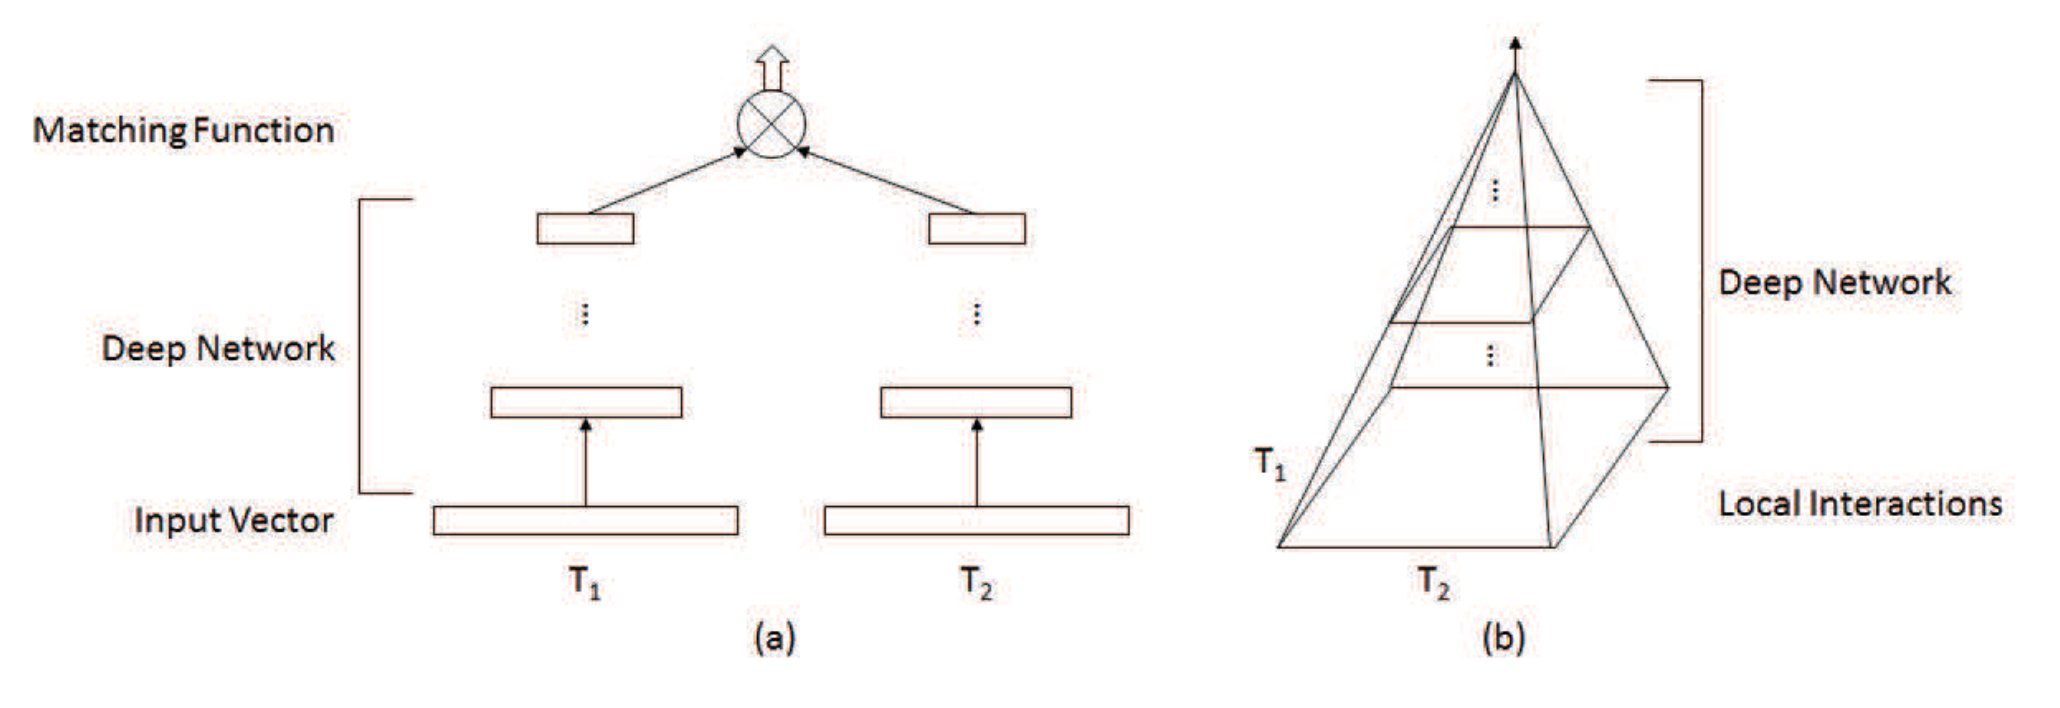
\includegraphics[width=5in]{deep_matching.png}
\caption{\cite{guo2017drmm}}
\label{fig:deep_matching}
\end{figure}

With the massive successes achieved by neural networks in many areas such as computer vision and natural language processing \cite{}, document retrieval, too, has witnessed a shift from non-neural methods to neural methods over the last few years.
Neural models have especially been instrumental in \myworries{improving} semantic matching in document retrieval.
Neural models developed to address the deep matching problem in document retrieval can be divided into two broad categories based on their underlying architecture: representation-based and interaction-based.
These architectures are illustrated at a high level in Figure \ref{fig:deep_matching}, and discussed at length in the following sections.

\subsubsection{Representation-based Models}

Representation-based approaches first construct a representation from the input vectors for the query and document with a deep neural network, and then perform matching between these representations (see  Figure \ref{fig:deep_matching}).
One set of such models loan the concept of word embeddings from natural language processing to represent query and documents.
Some of the most popular pretrained English word embeddings include word2vec \cite{mikolov2013distributed} trained on  Google News, GloVe \cite{pennington2014glove} on Common Crawl, Wikipedia and Twitter, and fastText \cite{bojanowski2017enriching} on English webcrawl and Wikipedia.
Word embeddings can be learned from scratch for a specific corpus or pretrained over large corpora and reused, leading to significant improvements over the former \cite{turian2010word}.
There has also been some effort in learning word embeddings to directly capture relevance matching \cite{DBLP:journals/corr/ZamaniC17, ganguly2015word} rather than linguistic features as in word2vec \cite{mikolov2013distributed} or GlovE \cite{pennington2014glove}.

Other representation-based architectures explore alternative ways to represent text for effective retrieval.
DSSM (short for Deep Structured Semantic Models) \cite{huang2013learning} extends previously dominant latent semantic models \cite{blei2003latent, } to deep semantic matching for web search by projecting query and documents into a common low-dimensional space.
In order to accommodate a large vocabulary required by the task, the text sequences are mapped into character-level trigrams with a word hashing layer before computing a similarity matrix through dot product and softmax layers.
While shown effective on a private dataset comprised of log files of a commercial search engine, DSSM was criticized by Guo et al. \cite{guo2017drmm} for requiring too much training data to be effective.
Moreover, DSSM cannot match synonyms because it is based on the specific composition of words and not semantic proximity.
C-DSSM \cite{shen2014learning} was proposed as an extension to DSSM by replacing the multi-layer perceptron with a convolutional layer to devise semantic vectors for search queries and Web document.
By performing a max pooling operation to extract local contextual information at the n-gram level, a global vector representation is formed from the local features.
Shen et al. \cite{shen2014learning} demonstrate that both local and global contextual features are necessary for semantic matching for Web search.
While C-DSSM improves over DSSM by exploiting the context of each trigram, it still suffers from most of the same issues listed above.

\subsubsection{Interaction-based Models}

Interaction-based approaches capture local matching signals, and directly compute word-word similarity between query and document representations.
In contrast to more shallow representation-based approaches, this setup allows the deep neural network to learn more complex hierarchical matching patterns across multiple layers.
Some notable examples of these architectures include DRMM \cite{guo2017drmm}, KNRM \cite{xiong2017knrm} and DUET \cite{mitra2017learning}.
\myworries{Explicit benefit of each method?}
DRMM, which stands for Deep Relevance Matching Model, \cite{guo2017drmm} maps variable-length local interactions of query and document into a fixed-length matching histogram.
A feed forward matching network is used to learn hierarchical matching patterns from the histogram representation, and a matching score is computed for each term.
An overall matching score is obtained by aggregating the scores from each query term with a term gating network.
KNRM \cite{xiong2017knrm} similarly calculates the word-word similarities between query and document embeddings, but converts word-level interactions into ranking features with a novel kernel pooling technique.
Specifically, a feature vector for each word in the query is constructed from the similarity matrix with k-max pooling.
Ranking features are combined to form a final ranking score through a learning-to-rank layer.
Unfortunately, Xiong et al. \cite{xiong2017knrm} only report results on a private dataset consisting of search logs from Sogou, limiting comparison to other neural retrieval models.
Unlike DRMM and KNRM, the goal of DUET \cite{mitra2017learning} is to employ both local and distributed representations, therefore leveraging both exact matching and semantic matching signals.
DUET is composed of two separate deep neural networks, one to match the query and the document using a one-hot representation, and another using learned distributed representations, which are trained jointly.
The former estimates document relevance based on exact matches of the query terms in the document by computing an interaction matrix from one-hot encodings.
The latter instead performs semantic matching by computing the element-wise product between the query and document embeddings.
Their approach significantly outperform traditional baselines for web search with lots of clickthrough logs.

\subsubsection{Contextualized Language Models}

While the models introduced in Section \ref{neural-retrieval} successfully leverage semantic information to varying degrees, they are limited by the size and variability of available training data.
Ideally, these models would be trained on a large number of semantically and syntactically varied labeled query-document pairs; however, it is impractical to automatically gather a sufficient number of such training samples at scale.
For this reason, massively pretrained unsupervised language models hold promises for obtaining better query and document representations, and therefore, achieving unprecedented effectiveness at semantic matching without the need for more relevance information.
Section \ref{lm} outlines some of the most popular unsupervised language models that form the basis of effective retrieval architectures.
In general, these language models are deployed as re-rankers over an initial list of candidate documents retrieved with traditional term-matching techniques in Section \ref{non-neural-retrieval}.

Modeling relevance requires an understanding of the relationship between two text sequences -- the query and the document; traditionally language modeling does not suffice to capture such a relationship.
Fortunately, BERT facilitates such relevance classification by pre-training a binary next sentence prediction task based on its masking language model approach as discussed in Section \ref{lm}.
However, it is still not trivial to apply BERT to document retrieval because BERT was not designed to handle long spans of text, such as documents, given a maximum input length of 512 tokens.
Partly because of this inherent challenge, the majority of work on re-ranking with BERT has focused on 
passage re-ranking instead of document re-ranking.

Notably, Nogueira et al. \cite{nogueira2019passage} proposed to re-rank MS MARCO passages based on a simple re-implementation of BERT to learn a model of relevance, outperforming the previous state of the art by 27\% in MRR@10 and replacing the previous top entry in the leaderboard of the MS MARCO passage retrieval task.
Our neural model is inspired by the BERT re-implementation described in their paper.
Padigela et al. \cite{Padigela:1905.01758:2019} prioritize studying the reasons behind the gains that come with re-ranking MS MARCO passages with BERT.
To put re-ranking with BERT into perspective, they compared their BERT-based reranker to feature based learning to rank models such as RankSVM \cite{joachims2002optimizing} and a number of neural kernel matching models such as KNRM \cite{xiong2017knrm} and Conv-KNRM \cite{dai2018convolutional}, and conclude that  fine-tuning BERT is substantially more effective than either neural model.
They also test four hypotheses regarding the behavior of matching with BERT compared to BM25; specifically, with respect to term frequency and document length.

To our knowledge, Yang et al. \cite{yang2019simple} are the first to successfully apply BERT to ``ad hoc'' document retrieval.
They demonstrate that BERT can be fine-tuned to capture \myworries{relevance} matching by following the abovementioned approach on the TREC Microblog Tracks where document length does not pose an issue.
They further propose overcoming the challenge of long documents by applying inference on each individual sentence and combining the top scores to compute a final document score.
Their approach is motivated by user studies by Zhang et al. \cite{zhang2018effective} which suggest that the most relevant sentence or paragraph in a document provides a good proxy for overall document relevance.
The work of Yang et al. \cite{yang2019simple} paved the way for future work that culminated in this thesis.

More recently, MacAvaney et al. \cite{macavaney2019cedr} shifted focus from incorporating BERT as a reranker to using its representation capabilities to improve existing neural architectures.
By computing a relevance matrix between the query and each candidate document at each layer of a contextualized language model -- in particular, ELMo or BERT --  they report a high score of NDCG2@20 0.5381 on Robust04 by using combining CEDR (Contextualized Embeddings for Document Ranking) with KNRM \cite{xiong2017knrm}.
They also propose a joint model that combines the aforementioned classification mechanism of BERT into existing neural architectures.
They claim that this approach benefits from both deep semantic matching with BERT \textit{and} relevance matching with traditional ranking architectures.

A recent arXiv preprint by Qiao et al. \cite{Qiao:1904.07531:2019} also examines the performance and behavior of BERT when used as a reranker for passage ranking on MS MARCO and for document ranking on the TREC Web Track.
Their findings are consistent with those of Nogueira et al. \cite{nogueira2019passage} in that BERT outperforms previous neural models on the passage reranking task on MS MARCO.
For ad hoc document ranking, they explore using BERT both as representation-based and interaction-based rankers and in combination with KNRM \cite{xiong2017knrm} and Conv-KNRM \cite{dai2018convolutional}.
However, they find that their reranking TREC Web Track documents with BERT performs worse than Conv-KNRM and feature-based learning-to-rank models trained on user clicks in Bing's search log.
%"In comparison, TREC ad hoc tasks require different signals other than surrounding context: pre-training on user clicks is more effective than on surrounding context based signals."

\subsection{Comparison of Non-neural and Neural Methods}

Despite growing interest in neural models for document ranking, researchers have recently voiced concern as to whether or not they have truly contributed to progress~\cite{lin2019neural}, at least in the absence of large amounts of behavioral log data only available to search engine companies.
Some of the models discussed in this section are designed to address the web search task where a variety of other signals are available, such as large amounts of log data and the webgraph.
However, this is not the case for ``ad hoc'' document retrieval where the only available data is the document text, which is the main focus of this thesis.
This opinion piece by Lin~\cite{lin2019neural} also echoes the general skepticism concerning the empirical rigor and contributions of machine learning applications in Lipton et al. \cite{lipton2018troubling} and Sculley at al. \cite{sculley2018winner}.
%\myworries{In particular, Lin et al.~\cite{lin2019neural} lament that comparisons to weak baselines sometimes inflate the merits of certain neural information retrieval methods.}

\begin{figure}[b!]
\centering
  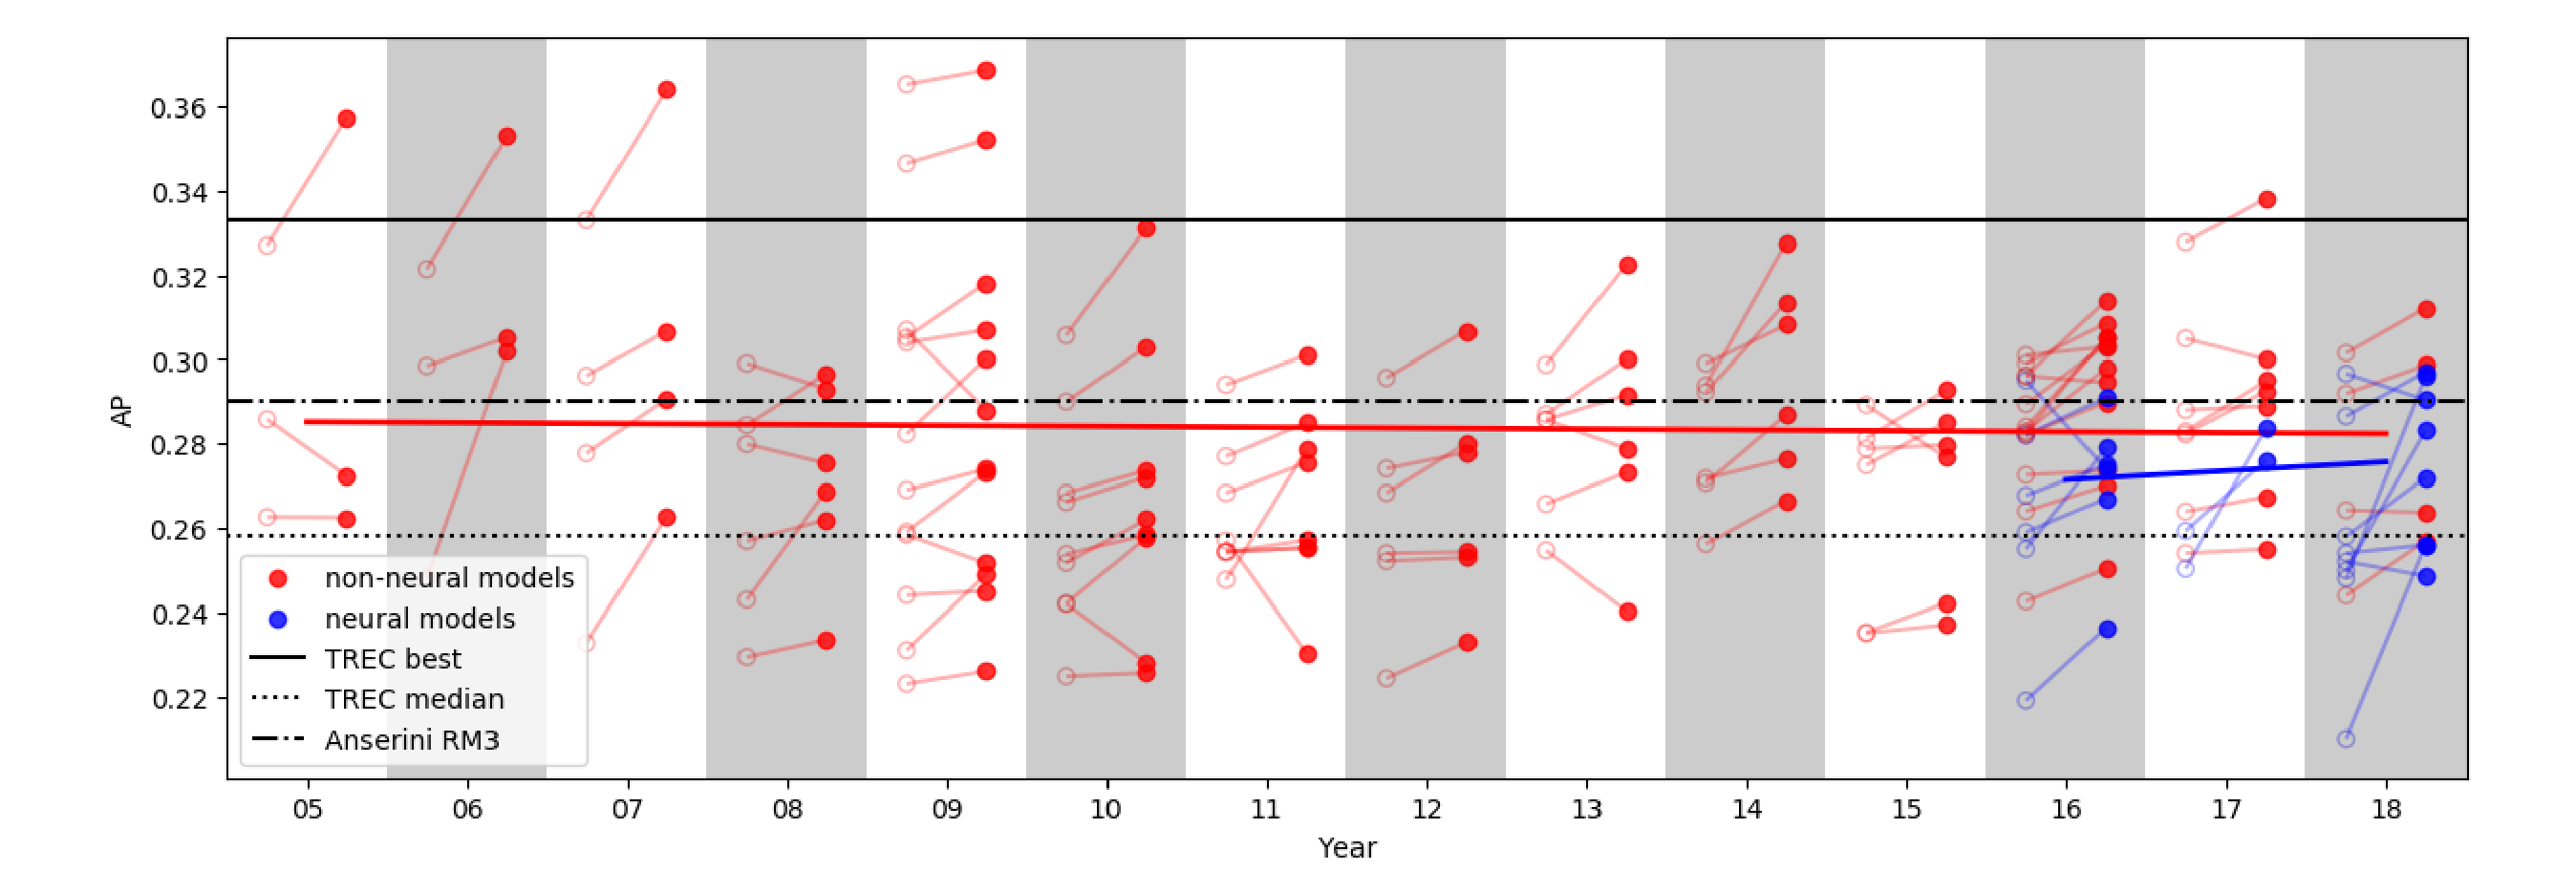
\includegraphics[width=6.5in]{neural_robust04.png}
\caption{...}
\label{fig:neural_robust04}
\end{figure}

To rigorously test this claim, Yang et al. \cite{Yang_etal_SIGIR2019} recently conducted a thorough meta-analysis of over 100 papers that report results on the TREC Robust 2004 Track.
Their findings are illustrated in Figure \ref{fig:neural_robust04} where the solid black line represents the best submitted run at 0.333, and the dotted black line the median TREC run at 0.258.
The other line is a RM3 baseline run with default parameters from the Anserini open-source information retrieval toolkit~\cite{Yang:2018:ARR:3289400.3239571} at AP 0.3903.
The untuned RM3 baseline is more effective than ~60\% of all studied papers, and ~20\% of them report results below the TREC median.
More surprisingly, only six of them report AP scores higher than the TREC best, with the highest being by Cormack et al.~\cite{Cormack:2009:RRF:1571941.1572114} in 2009 at AP 0.3686.
Their approach is based on building an ensemble of multiple TREC runs with reciprocal rank fusion.
Among the neural models, the highest encountered score is by Zamani et al.~\cite{zamani2018neural} in 2018 at AP 0.2971.
Deviating from the dominant approach of deploying neural models as rerankers, Zamani et al.~\cite{zamani2018neural} propose a standalone neural ranking model to learn a latent representation for each query and document, which is sparse enough to construct an inverted index for the entire collection.
However, their report result is still much lower than the TREC best and far below the best reported result of Cormack et al.~\cite{Cormack:2009:RRF:1571941.1572114}.
Overall, Figure \ref{fig:neural_robust04} displays no clear upward trend in terms of AP on Robust04 from 2005 to 2018.

%Yang et al. also implemented five recent neural retrieval models discussed above to evaluate their effectiveness on the ``ad hoc'' document retrieval task on the Robust04 dataset: DSSM, CDSSM, DRMM, KNRM and DUET.
%These models were selected because they were specifically designed for ``ad hoc'' document retrieval unlike some others designed to handle shorter texts?
%\myworries{All the models were trained on the documents in the baseline RM3 runs... details CV etc}
%Table \ref{tab:exp-robust04} displays the AP and NDCG@20 values of each run on the Robust04 dataset.
%The first two rows are taken from the original DRMM paper~\cite{guo2017drmm} and show their reported baseline and results; the other models do not report results on Robust04.
%The next row refers to the untuned RM3 baseline from Anserini.
%The following results refer to results from the neural models that were used to rerank the strong baseline, BM25+RM3, to gauge how much they actually contribute.
%Of the five models, only one -- DRMM -- is found to significantly improve over the baseline.

The other two collections, from the TREC Common Core 2017 (Core17) \cite{allan2017trec} and 2018 (Core18) \cite{}, that we evaluate our models on are not nearly as well-studied as Robust04.
Excluding runs that make use of past labels or require human intervention, the TREC best run on Core17 is \texttt{umass baselnrm} at AP 0.275 and on Core18 \texttt{uwmrg} at AP 0.276.
\myworries{describe...}
To our knowledge, Neural Vector Spaces for Unsupervised Information Retrieval by Van Gysel et al. \cite{Gysel:2018:NVS:3211967.3196826} represent the only major neural model evaluated on Core17.
While their approach has the advantage of not requiring supervised relevance judgements, their reported results are quite low.
Otherwise, evaluation of neural retrieval methods on both Core17 and Core18 has been limited.

\section{Evaluation Metrics}

Evaluation in information retrieval relies on the distinction between ``relevant'' and ``irrelevant'' documents with respect to an information need as expressed by a query.
A number of automatic evaluation metrics has been formalized specifically for ranking tasks, some of which are introduced below.

%The size of most document collections makes it infeasible for humans to manually judge the relevance of all documents.
%All relevant documents need to be labelled to prevent false negatives, i.e: treating documents which are in fact relevant as irrelevant.

\subsection{Mean Average Precision (MAP)}

Precision specifies what fraction of a set of retrieved documents is in fact relevant for a given query $ q $.
By extension, average precision (AP) expresses the average of the precision values obtained for the set of top $ k $ documents for the query.
Support that $ D = \{d_1, ..., d_{m_j}\} $ is the set of all relevant documents for a query $ q_j $, then AP can be formulated as:

\begin{equation}
AP = \frac{1}{m_j} \sum^{m_j} _{k = 1} P(R_{jk})
\end{equation}

where $ R_{jk} $ represents the set of top $ k $ ranked retrieval results.

The respective AP for each query $ q_{j} \in Q $ can be aggregated to obtain mean average precision (MAP) for the overall retrieval effectiveness in the form of a single-figure measure of quality across various recall levels:

\begin{equation}
MAP = \frac{\sum^{|Q|} _{j = 1} AP}{Q} = \frac{1}{Q} \sum^{|Q|} _{j = 1} \frac{1}{m_j} \sum^{m_j} _{k = 1} P(R_{jk})
\end{equation}

%\myworries{Meaning of MAP: To recapitulate, if the AP is 0.5, the relevant
%answer occurs at every second position. If the AP score is 0.3, the relevant answer occurs
%at every 3rd position and an AP score of 0.1 would mean that every 10th answer is correct.}

MAP is known to have especially good discrimination and stability compared to other evaluation metrics, which makes it the ideal choice for large text collections \cite{manning2010introduction}.
It is hence one of the standard metrics among the TREC community.

\subsection{Precision at k (P@k)}

While MAP factors in precision at all recall levels, certain applications may have a distinctly different notion for ranking quality.
Particularly in the case of web search, the user often only cares about the results on the first page or two.
This restriction essentially requires measuring precision at fixed low levels of retrieved results, i.e: top $ k $ documents -- hence the name for the metric ``precision at $ k $''.
On the one hand, it eliminates the need for any estimate of the size of the set of relevant documents because it is only concerned with the top documents.
However, it also produces the least stable results out of all evaluation metrics.
Moreover, precision at $ k $ does not average well because it is too sensitive to the total number of relevant documents for a query.

\subsection{Normalized Discounted Cumulative Gain (NDCG@k)}

Cumulative gain (CG) simply computes the sum of relevance labels for all the retrieved documents, treating the search results as an unordered set.
However, since a highly relevant document is inherently more useful when it appears higher up in the search results, CG has been extended to discounted cumulative gain (DCG).
Discounted cumulative gain (DCG) estimates the relevance of a document based on its rank among the retrieved documents.
The relevance measure is accumulated from top to bottom, discounting the value of documents at lower ranks.
NDCG at $ k $ measures DCG for the top $ k $ documents, normalizing by the highest possible value for a query; therefore, a perfect ranking yields NDCG equals 1.

NDCG is uniquely useful in applications with a non-binary notion of relevance, e.g: a spectrum of relevance.
This makes NDCG comparable across different queries:\
The NDCG values for all queries can be averaged to reliably evaluate the effectiveness of a ranking algorithm for various information needs across a collection.
Given a set of queries $ q_j \in Q $ and relevance judgements $ R_{dj} $ for a document $ d $:\

\begin{equation}
NDCG(Q, k) = \frac{1}{|Q|} \sum ^{|Q|} _{j = 1} Z_{kj} \sum ^k _{m = 1} \frac{2^{R(j, m)} - 1}{log_2 (1 + m)'}
\end{equation}

where $ Z_{kj} $ is the normalization factor.